\subsection{Forward Kinematic Equations of Fanuc 210F}



\subsubsection{Local Coordinate Reference Frames on the Fanuc 210F}

As described in \Autoref{sec:localRefFrame}, the local coordinate reference frames can also be attached to the Fanuc 210F as seen in \Autoref{fig:RefFrame}. For an overview how find the joints and links as well as the z-axis orientations see \Autoref{sec:jointsandlinks}. %\paragraph{Assignment of indvidual frames}
The assignment of individual frames can be found in appendix \Autoref{app:IndFrameAss}.\\

\begin{figure}[H]
	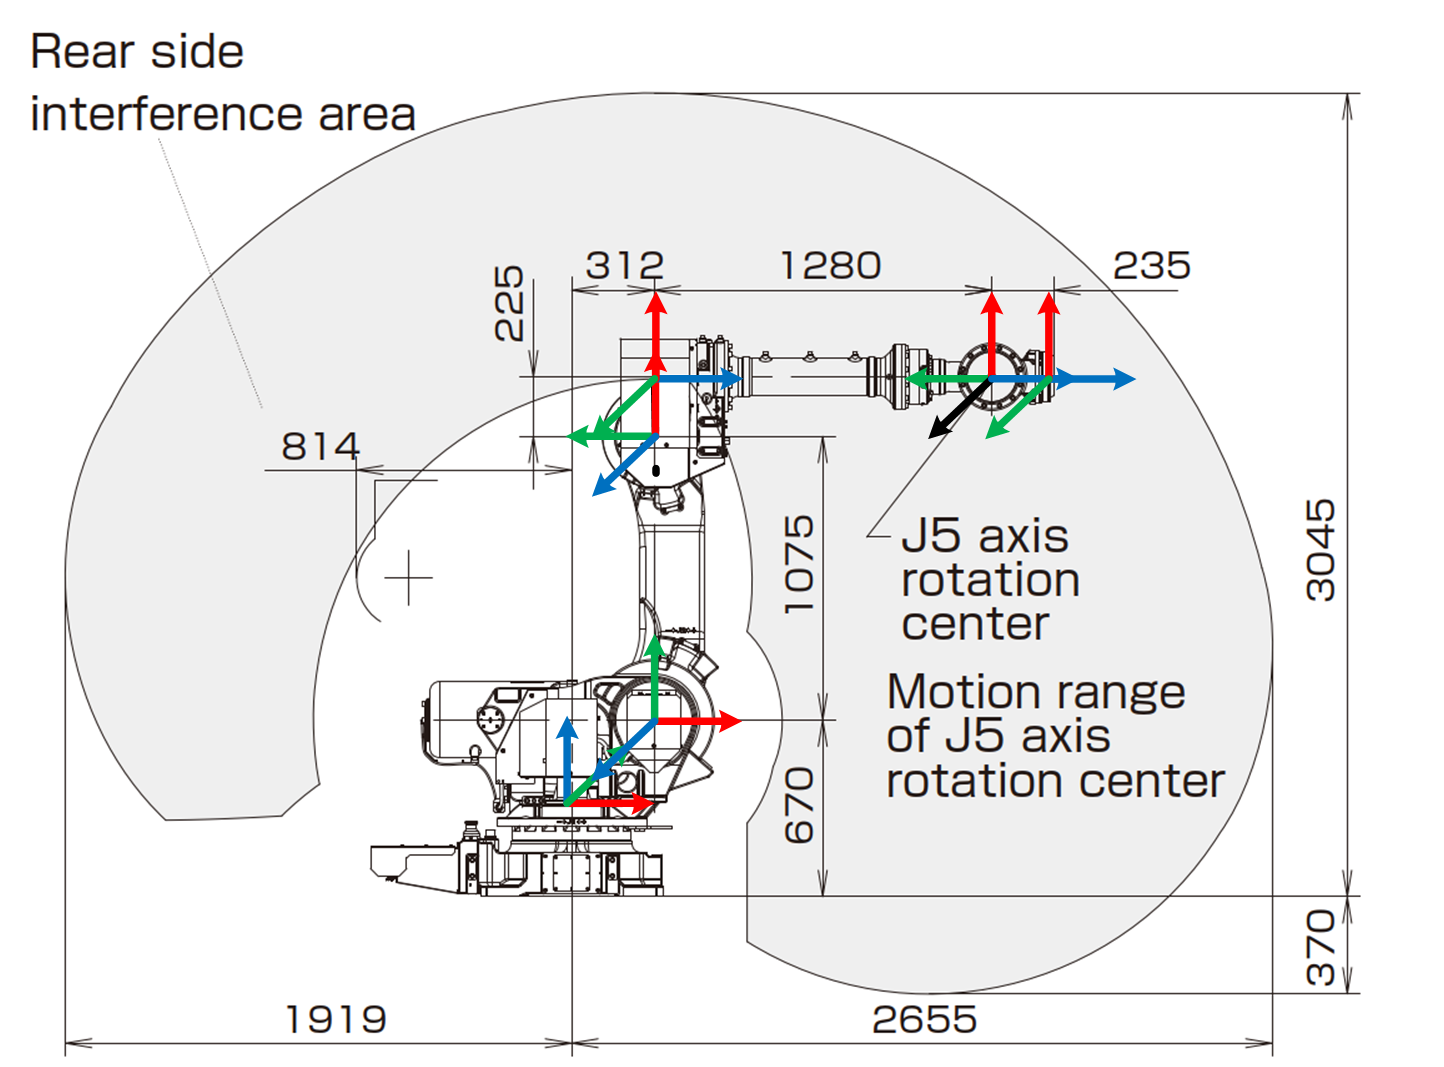
\includegraphics[
	width=1\linewidth,
	center,
	keepaspectratio,
	]{coordinateFrames/CoordinateFramesRobotStandardPose}
	\caption{Coordinate reference frames for Fanuc 210F in standard (Normal) pose}
	\label{fig:RefFrame}
\end{figure}






\medskip




\subsubsection{Establishing \ac{DH} Parameters on the Fanuc 210F}

As described in \Autoref{sec:DHparPerLink}, the \ac{DH}-Parameters can also be determined for the Fanuc 210F.
These parameters can be found with the help of the assigned coordinate frames as seen in \Autoref{fig:DH_Parameters_Fanuc210F}. For simplicity, only non-zero DH-parameters are shown in this figure.

\begin{figure}[h]
	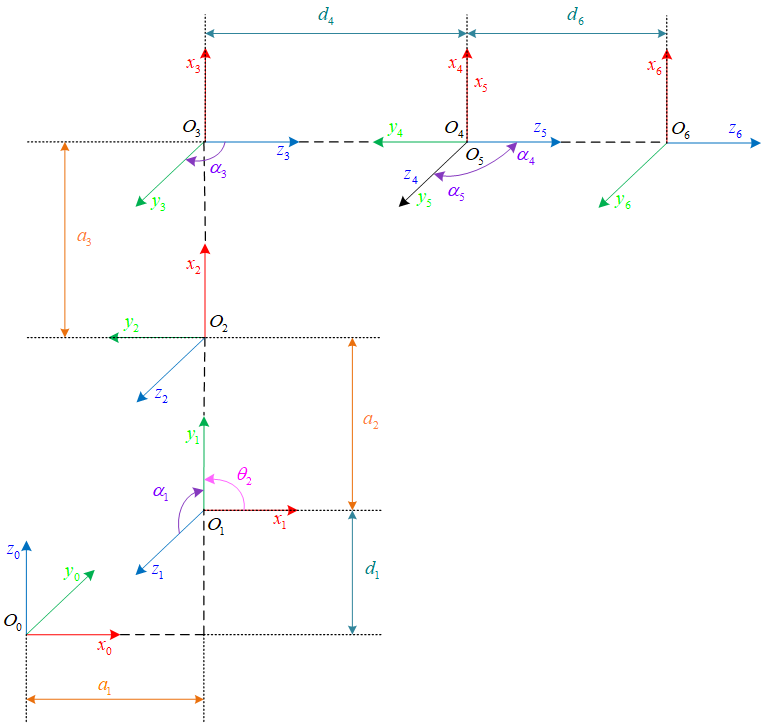
\includegraphics[
	width=1\linewidth,
	center,
	keepaspectratio,
	]{coordinateFrames/DH_Parameters_assignment}
	\caption{Assignment of DH-Parameters on the Fanuc 210F}
	\label{fig:DH_Parameters_Fanuc210F}
\end{figure}


To wrap this up, a summary of the DH-parameters for each link as follows from \Autoref{fig:DH_Parameters_Fanuc210F} can be found in \Autoref{table:DH-Parameter}.\\


%Generate tables easily with: % https://www.tablesgenerator.com/

\begin{table}[H]
	\centering
	\begin{tabular*}{0.5\textwidth}{|l||@{\extracolsep{\fill}}l|l|l|l|}
		\hline
		Link & \multicolumn{1}{l|}{$\theta_i$} & \multicolumn{1}{l|}{$d_i$} & \multicolumn{1}{l|}{$a_i$} & \multicolumn{1}{l|}{$\alpha_i$} \\ \hline\hline
		1 & $\theta_1$ & $d_1$ & $a_1$ & $\alpha_1$\\ \cline{1-5}
		2 & $\theta_2$ & 0     & $a_2$ & 0         \\ \cline{1-5}
		3 & $\theta_3$ & 0     & $a_3$ & $\alpha_3$\\ \cline{1-5}
		4 & $\theta_4$ & $d_4$ & 0     & $\alpha_4$\\ \cline{1-5}
		5 & $\theta_5$ & 0     & 0     & $\alpha_5$\\ \cline{1-5}
		6 & $\theta_6$ & $d_6$ & 0     & 0         \\ \cline{1-5}
		%\hline
	\end{tabular*}
	\caption{\acrfull{DH} Parameters for Fanuc 210F}
	\label{table:DH-Parameter}
\end{table}


\paragraph{Numeric values of DH-parameters}

As can be seen from \Autoref{table:DH-Parameter}, many \ac{DH}-parameters are zero due to a good choice of pose and coordinate frames. 
All angles are plus or minus 90°.

Most of the frames have translational transformations in either $\gls{a_i}$ or $\gls{d_i}$ direction with link 1 and 5 being the exception.
By lifting the base frame out of the joint, parameter $d_1$ could be set to zero as well (see \Autoref{fig:DH_Parameters_Fanuc210F}). For better understanding, the origin of the frame was originally kept inside the joint (see \Autoref{fig:RefFrameAbstract}).
Frame 5 shares the origin with frame 4, not requiring any translational movement.
Most of the frames are also rotated by 90 degree around the x-axis with link 2 and 6 being the exception. Frame 6 was chosen with the same orientation as frame 5. Frame 2 has the same x-axis orientation as link 1 because joints two and three are parallel. There is just a rotational transformation around the z-axis of 90°. This is only due to the standard pose of the robot, as theta is a variable.
For all coordinate frames theta is a variable, as all joints are revolute and none is translational. 

Besides the angle values for $\alpha_i$ which were easy to determine from the graphical interpretation in \Autoref{fig:DH_Parameters_Fanuc210F}, following numeric values need to be determined through measurements or drawings:\\
$d_1$, $d_4$, $d_6$ and 
$a_1$, $a_2$, $a_3$. 

%A great help to determine these values is fig \ref{fig:RefFrame}. This technical drawing was obtained from the data-sheet for all Fanuc R-2000iB series robots. 
With \Autoref{fig:RefFrame} following \ac{DH}-parameters can be obtained:

\begin{itemize}\label{item:DH-LinparamValues}
	\item[$a_1$=] 312 [\textit{mm}]
	\item[$a_2$=] 1075 [\textit{mm}]
	\item[$a_3$=] 225 [\textit{mm}]
	\item[$d_4$=] 1280 [\textit{mm}]
	\item[$d_6$=] 235 [\textit{mm}]
\end{itemize}

The parameter $d_1$ cannot be determined from this drawing. It can either be measured on the actual robot, or defined as zero, as frame zero can be freely moved along the z-axis. A value of zero would put the origin of the base frame on the same height as frame 1, simplifying subsequent steps. 
It must be clear though, that all referencing in the forward and backward kinematics will be relative to this point. 
A change of this point of reference can be added later simply by adding another transformation matrix for translational movement along the z-axis as seen in \cite{Paul1981RobotM}.\\
\\
This results in a table of numeric DH-parameters as seen in \Autoref{table:DH-Parameter_num}. The transformation $^{i-1}\hat{T}_i$ changes with only a single variable $\gls{theta_i}$ as all of the other quantities stay constant, and all joints are revolute.

\begin{table}[H]
	\centering
	\begin{tabular*}{0.5\textwidth}{|l||@{\extracolsep{\fill}}l|l|l|l|}
		\hline
		Link & \multicolumn{1}{l|}{$\theta_i$} & \multicolumn{1}{l|}{$d_i$} & \multicolumn{1}{l|}{$a_i$} & \multicolumn{1}{l|}{$\alpha_i$} \\ \hline\hline
		1 & $\theta_1$ & 0     & 312   & $\pi/2$  \\ \cline{1-5}
		2 & $\theta_2$ & 0     & 1075  & 0        \\ \cline{1-5}
		3 & $\theta_3$ & 0     & 225   & $\pi/2$  \\ \cline{1-5}
		4 & $\theta_4$ & 1280  & 0     & $-\pi/2$ \\ \cline{1-5}
		5 & $\theta_5$ & 0     & 0     & $\pi/2$  \\ \cline{1-5}
		6 & $\theta_6$ & 235   & 0     & 0        \\ \cline{1-5}
		%\hline
	\end{tabular*}
	\caption{Numeric values of Denavit Hartenberg Parameters for Fanuc 210F}
	\label{table:DH-Parameter_num}
\end{table}


\subsubsection{Calculate Homogeneous Transformation Matrices}

For further details on how to set up $R_z(\theta_i), T_z(d_i), T_x(a_i) and R_x(\alpha_i)$ and form the transformation matrix in  \Autoref{eq:TransformationMarix} see %chapter 1 "Homogeneous Transformations" in %"Robot manipulators: mathematics, programming, and control: the computer control of robot manipulators" 
\cite{Paul1981RobotM}, chapter 1. The basic techniques for setting up the translation and rotation matrices as well as how to combine them are described in that chapter .




\subsubsection{Forward Kinematic Equations on the 210F}
As shown in \Autoref{fig:zi_Axes}, the Fanuc 210F is a 6-\ac{DOF} robotic arm with \gls{N}=six revolute joints in series. 
Their orientation can be expressed in short form with 
\begin{equation}
(R\perp R\parallel R\perp R\perp R\perp R ) .
\end{equation}

With this and \Autoref{eq:matrixForm}, the complete transformation matrix can be derived in the form as described in \Autoref{ForKinEq}.
The intermediate steps to get the forward kinematic equations can be found in appendix \Autoref{sec:FWKinEqSteps}.

%\begin{dmath}
%	\label{eq:ForwardKinEquations_6DOF_shortIntext}
%	\phantom{	n_x =  }\\
%	{n_x=c_1(c_{23}(c_4c_5c_6-s_4s_6)-s_{23}s_5c_6)+s_1(s_4c_5c_6-c_4s_6)}\\
%	{n_y=s_1(c_{23}(c_4c_5c_6-s_4s_6)-s_{23}s_5c_6)-c_1(s_4c_5c_6-c_4s_6)} \\
%	{n_z=s_{23}(c_4c_5c_6-s_4s_6)-c_{23}s_5c_6} \\
%	{o_x=c_1(-c_{23}(c_4c_5s_6+s_4c_6)-s_{23}s_5s_6)-s_1(s_4c_5s_6-c_4s_6)} \\
%	{o_y=s_1(-c_{23}(c_4c_5s_6+s_4c_6)-s_{23}s_5s_6)+c_1(s_4c_5s_6-c_4s_6)} \\
%	{o_z=-s_{23}(c_4c_5s_6+s_4s_6)-c_{23}s_5s_6} \\
%	{a_x=c_1(c_{23}c_4s_5+s_{23}c_5)+s_1s_4s_5} \\
%	{a_y=s_1(c_{23}c_4s_5+s_{23}c_5)+c_1s_4s_5} \\
%	{a_z=s_{23}c_4s_5-c_{23}c_5} \\
%	{p_x=c_1(a_1+a_2c_2+a_3c_{23}+d_4s_{23}+d_6(c_{23}c_4s_5+s_{23}c_5))+d_6s_1s_4s_5} \\
%	{p_y=s_1(a_1+a_2c_2+a_3c_{23}+d_4s_{23}+d_6(c_{23}c_4s_5+s_{23}c_5))+d_6s_1s_4s_5} \\
%	{p_z=a_2s_2+a_3s_{23}-d_4c_{23}+d_6(s_{23}c_4s_5-c_{23}c_5)} \\
%\end{dmath}

\begin{subequations}\label{eq:ForwardKinEquations_6DOF_shortIntext}
	\begin{align}
		n_x&=c_1(c_{23}(c_4c_5c_6-s_4s_6)-s_{23}s_5c_6)+s_1(s_4c_5c_6-c_4s_6)\\
		n_y&=s_1(c_{23}(c_4c_5c_6-s_4s_6)-s_{23}s_5c_6)-c_1(s_4c_5c_6-c_4s_6) \\
		n_z&=s_{23}(c_4c_5c_6-s_4s_6)-c_{23}s_5c_6 \\
		o_x&=c_1(-c_{23}(c_4c_5s_6+s_4c_6)-s_{23}s_5s_6)-s_1(s_4c_5s_6-c_4s_6) \\
		o_y&=s_1(-c_{23}(c_4c_5s_6+s_4c_6)-s_{23}s_5s_6)+c_1(s_4c_5s_6-c_4s_6) \\
		o_z&=-s_{23}(c_4c_5s_6+s_4s_6)-c_{23}s_5s_6 \\
		a_x&=c_1(c_{23}c_4s_5+s_{23}c_5)+s_1s_4s_5 \\
		a_y&=s_1(c_{23}c_4s_5+s_{23}c_5)+c_1s_4s_5 \\
		a_z&=s_{23}c_4s_5-c_{23}c_5 \\
		p_x&=c_1(a_1+a_2c_2+a_3c_{23}+d_4s_{23}+d_6(c_{23}c_4s_5+s_{23}c_5))+d_6s_1s_4s_5 \\
		p_y&=s_1(a_1+a_2c_2+a_3c_{23}+d_4s_{23}+d_6(c_{23}c_4s_5+s_{23}c_5))+d_6s_1s_4s_5 \\
		p_z&=a_2s_2+a_3s_{23}-d_4c_{23}+d_6(s_{23}c_4s_5-c_{23}c_5)
	\end{align}
\end{subequations}

In \ref{eq:ForwardKinEquations_6DOF_shortIntext}, following notations are used:
$c_i = cos(\theta_i)$, $s_{ij}=sin(\theta_1+\theta_j)$.

%With matrix \ref{eq:matrixForm} , the forward kinematic equations can be formed:




These kinematic equations can be used to simulate the movements of the Fanuc 210F for a given set of joint-angles.



